\section{Monitoraggio del traffico di rete}

\subsection{Introduzione al monitoraggio di rete}

La raccolta di dati da fonti eterogenee è oggi un'operazione relativamente semplice;
la vera sfida risiede nell'interpretare ciò che viene raccolto, in particolare
nel dominio della sicurezza informatica, dove le minacce reali rappresentano
eventi statisticamente rari in un flusso di traffico altrimenti monotono.

Poiché la stragrande maggioranza del traffico è benigna e gli attacchi più pericolosi
sono rari e difficili da distinguere dal rumore di fondo, è necessario un framework
strutturato che integri raccolta, archiviazione e analisi in un sistema coeso.

\subsection{Architettura generale di un framework di analisi di rete}

Un framework di analisi di rete ha lo scopo di integrare dati provenienti da fonti eterogenee
per fornire una visione completa e contestualizzata degli eventi che si verificano
all'interno di un'infrastruttura.
Esso orchestra il flusso di informazioni dai sensori di rete fino alla console dell'analista,
abilitando sia analisi in tempo reale che indagini storiche approfondite.

L'architettura generale di tale framework si basa su diversi componenti interconnessi:

\begin{itemize}
\item \textbf{Sensor Network} (rete di sensori): è il punto di partenza,
responsabile della raccolta dei dati grezzi della rete, degli host e dei servizi.
\item I dati possono essere inviati a un sistema di \textbf{Real-time Processing}
(elaborazione in tempo reale) per analisi immediate,
come il rilevamento di frame anomali o la generazione di log.
\item Contemporaneamente, i dati confluiscono nel \textbf{Repository},
il cuore del sistema di archiviazione, che a sua volta si suddivide in:
\begin{itemize}
\item \textbf{Archive}: deposito per i dati degli eventi.
\item \textbf{Annotation}: contenitore per i dati di arricchimento.
\item \textbf{Knowledge Base} (KB): base di conoscenza specifica dell'organizzazione.
\end{itemize}
\item Il sistema di \textbf{Query Processing} (elaborazione delle interrogazioni)
attinge al repository per permettere agli analisti di effettuare ricerche complesse
e sintetizzare le informazioni.
\item Infine, la \textbf{Console} funge da interfaccia di interazione utente,
permettendo di visualizzare i risultati delle analisi in tempo reale e delle interrogazioni,
e di interagire con il sistema.
\end{itemize}

\begin{figure}[H]
    \centering
    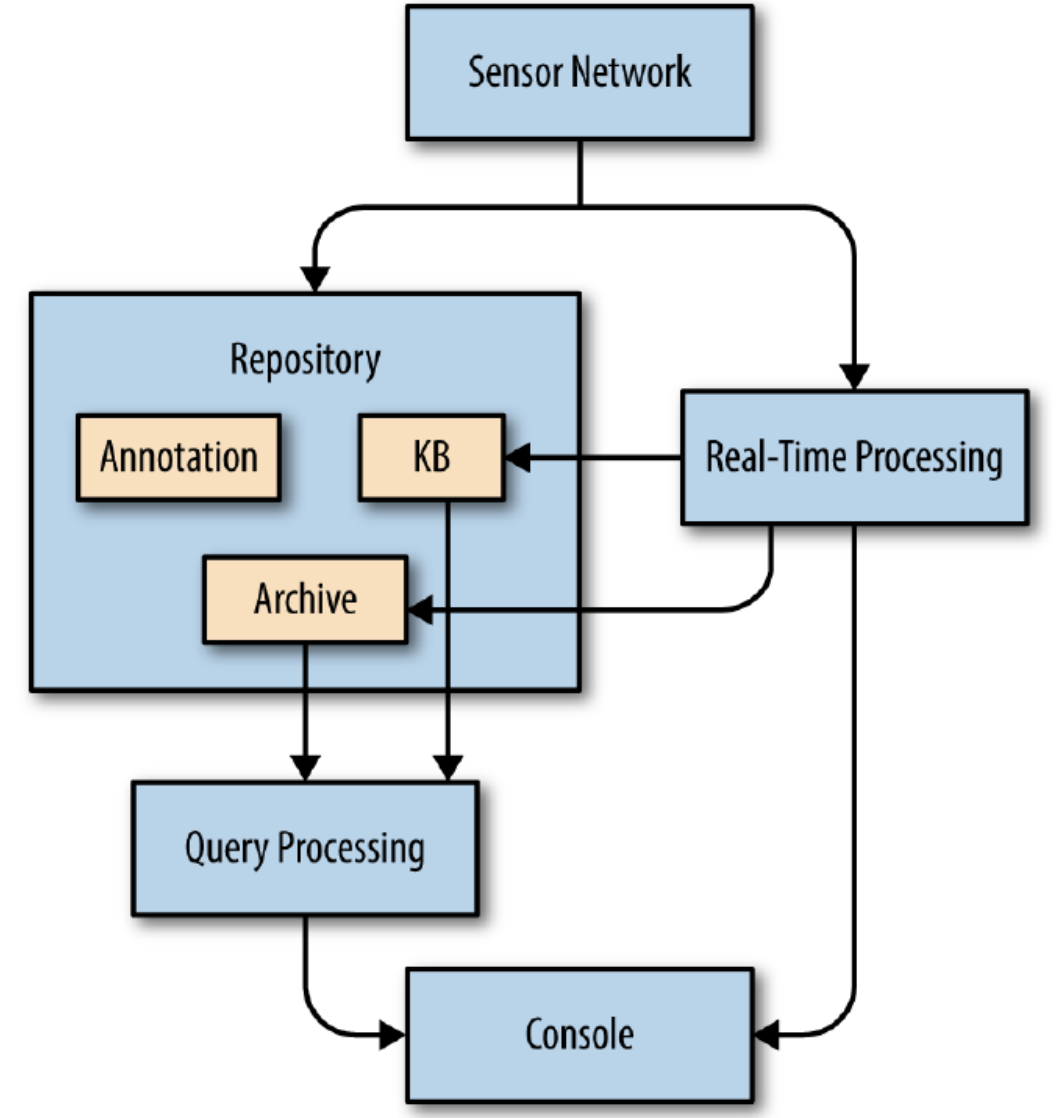
\includegraphics[width=0.5\textwidth]{img/frameworkAnalisi.png}
\end{figure}

\paragraph{Repository}

Il repository è il componente di archiviazione per tutti i dati che non vengono elaborati in streaming.
La sua progettazione deve rispondere a tre questioni fondamentali:

\begin{enumerate}
\item \textbf{Orizzonte Temporale}: Quanto a lungo conservare i dati? ne dipende un impatto sui costi 
e sulle capacità di storage necessarie.
\item \textbf{Strategie di Accesso}: Come differenziare l'accesso ai dati recenti e vecchi? Tipicamente 
si usano storage ad alte prestazioni per dati recenti, mentre quelli vecchi vengono spostati
in supporti meno performanti a basso costo.
\item \textbf{Aggiornamento delle Stime}: Con quale frequenza rivedere le stime di archiviazione? Il volume 
del traffico di rete è in costante cresciata, necessitando un riesame periodico delle encessità di storage
per evitare saturazioni.
\end{enumerate}

\paragraph{Archive}

L'archive è il deposito dedicato ai dati degli eventi.
Questi possono includere una vasta gamma di informazioni, come:

\begin{itemize}
\item \textbf{Dati di traffico di rete}: log di NetFlow, catture complete dei pacchetti (pcap).
\item \textbf{Informazioni di sistema}: statistiche sui processi, sull'utilizzo del file system,
report di antivirus.
\item \textbf{Log di sistema}: log dei server web, informazioni di syslog.
\end{itemize}

Una caratteristica chiave dell'archive è che i suoi dati sono \textbf{immutabili}:
una volta scritti, non vengono aggiornati.
Questo lo rende l'ambiente ideale per eseguire analisi forensi e storiche,
garantendo la coerenza e l'integrità delle evidenze.
Per ottimizzare lo spazio, per i dati più datati è spesso conveniente conservare
solo i risultati post-elaborazione, anziché i dati grezzi completi.

\paragraph{Annotation}

I dati di annotazione sono informazioni supplementari utilizzate per arricchire
e contestualizzare i dati presenti nell'archivio.
Esempi comuni includono feed di threat intelligence, dati di geolocalizzazione,
indicatori di reputazione degli IP e risoluzioni DNS.

A differenza dei dati di evento, che sono puntuali nel tempo, i dati di annotazione
possiedono una validità temporale.
Ad esempio, un indirizzo IP può appartenere a un'organizzazione dal 5 al 10 marzo
e a un'altra dall'11 marzo in poi.
Durante un'analisi, è di fondamentale importanza coordinare correttamente
queste informazioni temporali per attribuire a un evento l'entità corretta.

\paragraph{Knowledge Base (KB)}

La knowledge base è un insieme di informazioni e valutazioni specifiche
dell'organizzazione, costruite e accumulate nel tempo.
Contiene dati pertinenti esclusivamente all'ambiente target, come:

\begin{itemize}
\item Inventari degli asset di rete e dei sistemi.
\item Dati relativi al personale (es: ruoli, responsabilità).
\item Calendari interni (es: di manutenzione).
\end{itemize}

I dati della KB sono tipicamente non strutturati, di dimensioni relativamente ridotte,
e spesso gestiti e moderati direttamente dal personale interno.

\paragraph
{Storage System}

Il sistema di storage per il monitoraggio di rete non è un sistema di gestione
di database relazionali (RDBMS) tradizionale.
Mentre un RDBMS è progettato per interazioni bidirezionali tra molti utenti
e il database, un sistema di monitoraggio ha un modello di accesso diverso:
molti sensori scrivono dati verso un collettore centrale (log collector),
e un numero limitato di utenti/analisti legge.
In questo contesto, la consistenza transazionale tipica degli RDBMS
non è la priorità principale.

\paragraph{Query Processing}

Il sistema di query processing è un ambiente che consente di sintetizzare
i dati provenienti da molteplici fonti (archive, annotation, KB)
per fornire un contesto completo all'analisi.
Permette agli analisti di correlare informazioni diverse per costruire
un quadro d'insieme.
Le prestazioni e la capacità di gestire interrogazioni concorrenti
sono fattori chiave per la sua usabilità ed efficacia.

\paragraph{Real-time Processing}

L'elaborazione in tempo reale comprende tutte le analisi eseguite sui dati
man mano che vengono acquisiti dai sensori, prima ancora che vengano
archiviati in modo definitivo. Esempi di tali elaborazioni sono:

\begin{itemize}
\item Il signature matching per il rilevamento di pattern noti
(ad esempio, tramite strumenti come Snort o Suricata).
\item Analisi delle prestazioni per individuare anomalie.
\item La generazione di log strutturati a partire da dati grezzi.
\end{itemize}

Come regola di progettazione, l'elaborazione in tempo reale dovrebbe essere
distinta da quella delle query. Il suo scopo è riassumere o pre-elaborare i dati
per ridurre il carico sul sistema di query e fornire alert immediati.

Questo framework completo dipende interamente dalla qualità e dalla copertura
dei dati forniti dal suo componente di input prioritario: la rete di sensori.

\subsection{La rete di sensori (Sensor Network)}

La rete di sensori è il fondamento di qualsiasi sistema di monitoraggio.
È l'insieme di tutti i dispositivi di raccolta dati responsabili
dell'acquisizione delle informazioni grezze che alimentano l'intero
framework di analisi. La sua progettazione e il suo posizionamento
strategico sono cruciali per la visibilità e l'efficacia del monitoraggio.

I sensori possono essere classificati in base alla loro origine:

\begin{itemize}
\item \textbf{Network Sensing}: dispositivi che osservano direttamente
il traffico di rete, come Network Intrusion Detection Systems (NIDS),
firewall, e sensori di flusso (NetFlow) o di pacchetti (pcap).
\item \textbf{Host-based Sensing}: software installato sui singoli host,
come antivirus (AV) e Host-based Intrusion Detection Systems (HIDS).
\item \textbf{Service Sensing}: applicazioni che generano log relativi
ai servizi che erogano, come server web (log HTTP) o sistemi
centralizzati di log (syslog).
\end{itemize}

È importante distinguere questa raccolta passiva dal sensing attivo,
che viene eseguito su base ad hoc con strumenti come ping, traceroute
o Nmap per mappare la rete o verificare la connettività,
e non è parte integrante della rete di sensori permanente.

La progettazione di una rete di sensori solleva diverse questioni chiave:

\begin{enumerate}
\item \textbf{Trasporto dati}: i dati raccolti verranno trasportati
in-band (sulla stessa rete di produzione) o out-of-band
(su una rete dedicata)? Per volumi elevati di dati, è consigliabile
considerare VLAN dedicate per non impattare sulle performance
della rete principale.
\item \textbf{Archiviazione dati}: dove vengono memorizzati i dati?
Dati di riepilogo come NetFlow possono essere archiviati centralmente,
mentre dati grezzi e voluminosi come le catture di pacchetti possono
essere registrati localmente dai sensori e recuperati solo quando necessario.
\item \textbf{Meta-monitoring}: come si monitorano i sensori stessi?
L'integrità e il corretto funzionamento della rete di sensori
devono essere verificati costantemente.
\end{enumerate}

Dalla necessità di utilizzare sensori multipli e di diverso tipo,
emerge la complessità di gestire dati eterogenei. Per affrontare
questo problema è utile un modello di classificazione che aiuti
a categorizzare i sensori in base a posizione, dominio e azione.

\subsubsection{Classificazione dei sensori: un modello a tre attributi}

Per gestire la complessità derivante dall'impiego di sensori eterogenei,
è utile un sistema di classificazione basato su tre attributi chiave:
\textit{vantage} (posizione), \textit{domain} (dominio) e \textit{action} (azione).

Questo modello fornisce un metodo strutturato per categorizzare i sensori
in base a come gestiscono i dati, aiutando a comprendere i punti di forza
e le debolezze di ciascuno.

\begin{itemize}
\item \textbf{Domain (dominio)}: descrive il tipo di informazioni fornite
dal sensore (dove e come i dati sono raccolti).
\item \textbf{Vantage (posizione)}: indica come il posizionamento del sensore
all'interno della rete influenza la sua capacità di osservare gli eventi.
\item \textbf{Action (azione)}: definisce come il sensore interagisce con
i dati che raccoglie (ad esempio: li riporta, li sintetizza o agisce su di essi).
\end{itemize}

Questi attributi sono fondamentali perché aiutano a definire le sfide
che la raccolta dati pone alla validità delle conclusioni di un analista.
Per validità si intende la robustezza degli argomenti basati sui dati,
ovvero la certezza che le conclusioni derivino logicamente dalle premesse
e siano supportate dalle evidenze raccolte.

\subsubsection{Analisi del dominio (Domain)}

Il dominio descrive il tipo di informazioni che un sensore è in grado
di fornire. Sensori posizionati nello stesso punto, ma appartenenti
a domini diversi, offriranno prospettive differenti sullo stesso evento.
I domini principali sono:

\begin{itemize}
\item \textbf{Network}: i sistemi di questo dominio operano a livello di rete
e forniscono dati in tempo reale, basandosi sui singoli pacchetti.
Le fonti di dati tipiche sono le catture complete (pcap) e i metadati
sui flussi (NetFlow), mentre l'identità degli attori di rete è definita
tramite indirizzi IP e MAC.
\item \textbf{Service}: questi sensori raccolgono informazioni dai log
generati dai servizi (server web, database). L'osservazione avviene
in tempo reale ma è basata sugli eventi registrati dall'applicazione.
L'identità può essere un indirizzo IP, ma più spesso si basa su
identificatori specifici del servizio, come gli username.
\item \textbf{Host}: opera a livello di singolo sistema operativo,
raccogliendo dati in modo asincrono. Le fonti includono informazioni
sullo stato del sistema (processi, file aperti) e alert generati
da software di sistema (antivirus). L'identità è multiforme, potendo
includere indirizzi IP/MAC, ma anche identificatori univoci di sistema
come UUID.
\item \textbf{Active}: questo dominio si riferisce ai dati raccolti
tramite azioni esplicite e guidate dall'utente, come le scansioni di
rete (network scanning). A differenza degli altri domini, il timing
non è continuo ma dipende dall'iniziativa dell'analista. L'identità
è legata all'indirizzo IP e a identificatori di servizio.
\end{itemize}

\subsubsection{Analisi per posizione (Vantage)}

Il vantage (posizione) di un sensore descrive quali pacchetti è in grado
di osservare in un punto specifico della topologia di rete
(ad esempio: un link, un router, uno switch).
Sensori con vantage diversi possono vedere parti diverse dello stesso
evento, portando a conclusioni potenzialmente incomplete se non correlate.

La selezione dei punti di osservazione ottimali segue un processo in tre fasi:

\begin{enumerate}
\item Acquisire una mappa della rete e una lista dei punti in cui
è possibile installare strumentazione.
\item Determinare i vantage point potenziali, identificando per ogni
punto cosa è possibile vedere (traffico a livello L2, IP, L4
o applicativo).
\item Determinare la copertura ottimale, scegliendo un insieme di punti
che garantisca il monitoraggio desiderato con una ridondanza minima.
\end{enumerate}

La ridondanza può essere ulteriormente limitata tramite l'applicazione
di regole di filtraggio.

\paragraph{Vantage a livello Data Link}

A livello di data link (L2), la visibilità dipende dalla tecnologia di rete.

\begin{itemize}
\item \textbf{Link condiviso (hub o wireless)}: quando A invia un pacchetto
a B, tutti gli host sullo stesso segmento (C e D) vedono il pacchetto.
Tuttavia solo il destinatario B lo elabora. Un sensore (ad esempio D)
può registrare tutto il traffico.

\begin{figure}[H]
    \centering
    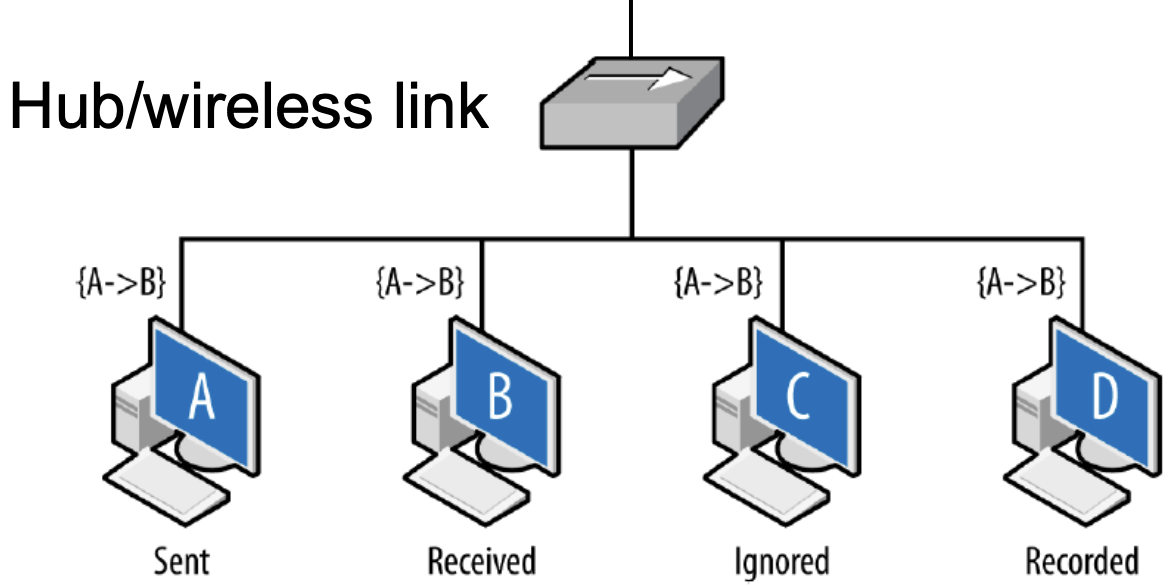
\includegraphics[width=0.5\textwidth]{img/vantageLink.png}
\end{figure}

\item \textbf{Su uno switch}: gli switch inoltrano il traffico solo sulla
porta del destinatario. Se A invia un pacchetto a B, gli host C e D
non vedono nulla. Per monitorare il traffico, è necessario configurare
una \textit{porta speculare} (mirrored port), che copia tutto il traffico
di una o più porte verso una porta a cui è collegato il sensore.
Un'alternativa hardware sono i \textit{physical tap}.

\begin{figure}[H]
    \centering
    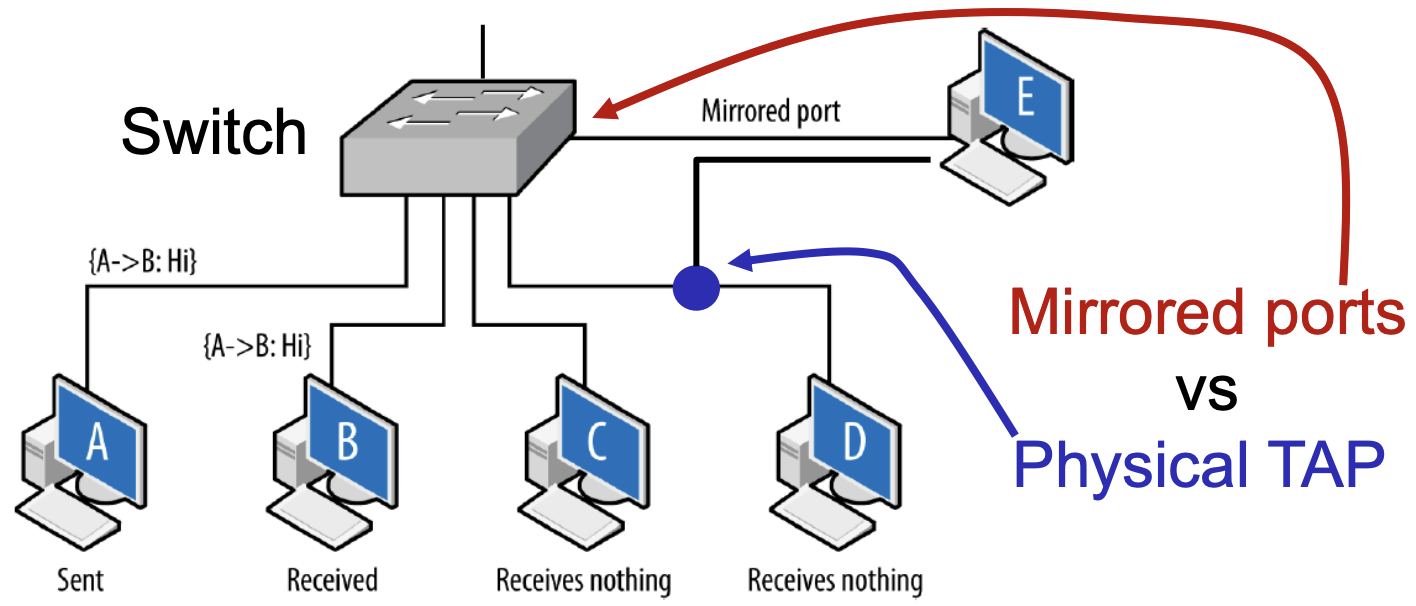
\includegraphics[width=0.5\textwidth]{img/vantageSwitch.png}
\end{figure}

\end{itemize}

\paragraph{Vantage a livello IP}

A livello IP (L3), emergono ulteriori complessità che possono compromettere
la validità dell'analisi.

\begin{itemize}
\item \textbf{Routing asimmetrico}: il percorso di andata e ritorno tra due host
può essere diverso. Nessun singolo sensore ha una visione completa della sessione,
rendendo difficile l'analisi dello stato della connessione.
\item \textbf{Valori TTL (Time-to-Live)}: il TTL di un pacchetto diminuisce ad
ogni hop. Un pacchetto con TTL troppo basso viene scartato prima di raggiungere
un certo sensore, che quindi non lo vedrà mai.

\begin{figure}[H]
    \centering
    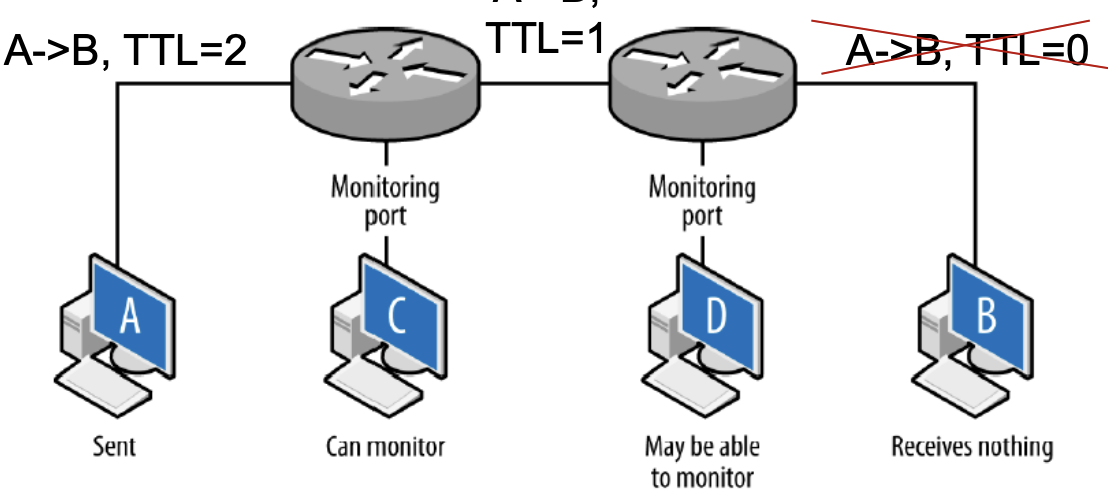
\includegraphics[width=0.5\textwidth]{img/vantageTTL.png}
\end{figure}

\item \textbf{Middlebox}: dispositivi intermedi come NAT, proxy e firewall
alterano l'indirizzo IP sorgente (SIP) e la porta sorgente (Sport) dei pacchetti.
Senza accedere ai log del middlebox, è impossibile correlare il traffico esterno
con il traffico interno. Le sfide introdotte riguardano:
\begin{itemize}
\item \textbf{Identity}: l'identità originale di un host viene mascherata o
manipolata, rendendo difficile risalire alla fonte.
\item \textbf{Causality}: l'ordine degli eventi osservati dopo il middlebox
potrebbe non corrispondere a quello precedente.
\item \textbf{Aggregation}: un'unica identità (IP pubblico) può essere usata
contemporaneamente da più host interni.
\item \textbf{Consistency}: la stessa identità può cambiare nel tempo
(esempio: un IP assegnato dinamicamente via DHCP).
\item \textbf{Encryption}: il traffico crittografato (esempio: VPN) impedisce
l'ispezione del payload.
\end{itemize}
\end{itemize}

Dispositivi diversi introducono sfide differenti: un NAT introduce problemi di
Identity, Aggregation e Consistency; un DHCP server impatta su Identity e
Consistency; un load balancer può alterare Causality e Consistency; un proxy
introduce le stesse sfide del NAT più Causality; una VPN introduce Identity,
Aggregation, Consistency ed Encryption.
Questo dimostra che, senza accesso diretto ai log dei middlebox, qualsiasi
analisi di traffico osservato esternamente è intrinsecamente incompleta
e potenzialmente fuorviante.

\subsubsection{Analisi per azione (Action)}

L'azione di un sensore descrive come esso interagisce con i dati che raccoglie.
Esistono tre tipi principali di azione:

\begin{enumerate}
\item \textbf{Report}: un sensore di tipo \textit{report} fornisce semplicemente
informazioni su tutti i fenomeni che osserva. È fondamentale per stabilire una
baseline del comportamento normale della rete e per sviluppare nuove fonti di
rilevamento degli attacchi. Esempi includono collettori NetFlow, tcpdump e
log dei server.
\item \textbf{Event}: un sensore di tipo \textit{event} analizza una o più
fonti di dati per produrre un evento che sintetizza le statistiche rilevate.
A differenza del sensore di report, non mostra tutto ma solo ciò che ritiene
significativo. Esempi includono gli Intrusion Detection Systems (IDS) e gli
antivirus, che possono agire come ``scatole nere'' che generano alert in base
a logiche interne complesse.
\item \textbf{Control}: un sensore di tipo \textit{control} va oltre la semplice
segnalazione: modifica o blocca attivamente il traffico quando rileva un evento.
Esempi sono gli Intrusion Prevention Systems (IPS), i firewall e i sistemi
antispam.
\end{enumerate}

In condizioni normali, il sensore Report (R) inoltra l'osservazione, mentre
Event (E) e Control (C) non producono alert. In presenza di un attacco, R
si limita a registrarlo, E genera un avviso (``We're attacked!''), e C blocca
attivamente il traffico malevolo impedendogli di raggiungere la destinazione.

\subsection{Formati dei dati e protocolli di monitoraggio}

Nel monitoraggio di rete vengono utilizzati diversi formati di dati, ciascuno
con i propri punti di forza. I principali includono:
\begin{itemize}
\item Catture di pacchetti LIVE o OFFLINE (file PCAP): offrono il massimo
livello di dettaglio.
\item Dati pre-elaborati come NetFlow o sFlow: utili per dashboard e
monitoraggio delle performance.
\item Dati basati su flussi (NetFlow): forniscono un ottimo compromesso
tra dettaglio e volume di dati.
\end{itemize}

\subsubsection{NetFlow}

NetFlow è contemporaneamente un protocollo di comunicazione, un formato dati
e un'applicazione, originariamente sviluppata da Cisco, utilizzata per raccogliere
metadati sui flussi di traffico IP che attraversano un dispositivo di rete.

L'architettura di base è semplice: un dispositivo abilitato a NetFlow
(come un router o uno switch), detto \textbf{Flow Exporter}, genera metadati
a livello di interfaccia e li invia a un server centrale, il \textbf{Flow Collector}.
Il valore di NetFlow risiede nella sua capacità di fornire un riepilogo compatto
delle sessioni di traffico, estremamente utile per analizzare throughput,
packet loss, congestione e potenziali pattern di sicurezza, in un formato
molto più leggero rispetto alla cattura completa dei pacchetti.

Al centro di NetFlow c'è il concetto di \textbf{flow} (flusso): un'approssimazione
di una sessione TCP. Poiché un router non può gestire i numeri di sequenza di
tutte le sessioni TCP come farebbe un endpoint, raggruppa i pacchetti che
condividono gli stessi indirizzi L3/L4 e sono vicini nel tempo, considerandoli
parte dello stesso flusso.

L'architettura NetFlow si compone di tre elementi principali:

\begin{itemize}
\item \textbf{Flow Exporter}: il dispositivo di rete (router/switch) che osserva
il traffico, genera i record dei flussi e li esporta.
\item \textbf{Flow Collector}: il server che riceve, archivia e pre-elabora
i record dei flussi inviati dagli exporter.
\item \textbf{Flow Analyzer}: l'applicazione software che analizza i dati
raccolti, trasformandoli in report, grafici e alert per gli analisti.
\end{itemize}

Un flusso unidirezionale è definito da un insieme minimo di attributi:
\begin{itemize}
\item Interfaccia di input.
\item Indirizzi IP sorgente e destinazione.
\item Porte sorgente e destinazione (L4).
\item Protocollo di livello 3 (esempio: TCP, UDP).
\item Campo Type of Service (ToS).
\end{itemize}

Un record di flusso viene esportato verso il collector quando si verifica
una delle seguenti tre condizioni:
\begin{enumerate}
\item \textbf{Inattività}: il flusso è inattivo per un periodo di tempo
predefinito (nessun nuovo pacchetto ricevuto).
\item \textbf{Lunga durata}: il flusso è attivo da più tempo di un timer
preconfigurato (per evitare che flussi molto lunghi non vengano mai esportati).
\item \textbf{Terminazione TCP}: viene osservato un flag TCP che indica la
fine della connessione (FIN o RST).
\end{enumerate}

\paragraph{Dettagli su NetFlow v5}

Nella versione 5 di NetFlow, il record del flusso viene incapsulato in un
datagramma UDP e inviato al collector. Un tipico record v5 include metadati
L3/L4, contatori di pacchetti e byte, timestamp di inizio e fine, interfacce
di input/output, flag TCP aggregati e informazioni di routing BGP.

I campi possono essere raggruppati logicamente:
\begin{itemize}
\item \textbf{Campi copiati dagli header}: \texttt{srcaddr} (IP sorgente),
\texttt{dstaddr} (IP destinazione), \texttt{srcport} e \texttt{dstport}
(porte TCP/UDP), \texttt{prot} (protocollo IP), \texttt{tos}
(Type of Service).
\item \textbf{Campi di riepilogo del traffico}: \texttt{packets} e
\texttt{dOctets} (contatori totali di pacchetti e byte a livello 3),
\texttt{first} e \texttt{last} (timestamp del primo e dell'ultimo pacchetto
nel flusso, relativi all'uptime del router).
\item \textbf{Flag TCP}: campo \texttt{TCP\_FLAGS} contenente l'OR logico
di tutti i flag TCP visti nel flusso. Per una sessione TCP completa,
saranno quasi sempre attivi SYN, FIN e ACK.
\item \textbf{Campi di routing}: indirizzo del nexthop, indici delle
interfacce di input/output, Autonomous System sorgente e destinazione
(\texttt{src-as}, \texttt{dst-as}) e relative maschere di rete.
\end{itemize}

\paragraph{Evoluzione di NetFlow}

NetFlow v5 è oggi uno standard obsoleto, principalmente perché limitato a IPv4.
L'evoluzione ha portato a \textbf{NetFlow v9}, uno standard flessibile basato
su template che permette agli amministratori di definire quali campi includere
nei record. La standardizzazione IETF di questo approccio è nota come
\textbf{IPFIX} (o NetFlow v10), che include pieno supporto a IPv6 e campi
specifici per il monitoraggio di ambienti con NAT.

\paragraph{Problematiche di generazione NetFlow}

La generazione di record NetFlow può avvenire in due modi:

\begin{itemize}
\item \textbf{Generazione su appliance}: sebbene integrata nel dispositivo,
questa modalità presenta diverse sfide. La mancanza di standardizzazione
tra vendor rende difficile avere configurazioni uniformi. Inoltre la
generazione di NetFlow può causare problemi di performance sui router,
specie sui modelli più datati. Le possibili soluzioni includono ridurre
la priorità del processo (rischiando di perdere record), usare hardware
dedicato (costoso) o applicare il campionamento (sconsigliato per l'analisi
di sicurezza, poiché potrebbe far perdere eventi critici).
\item \textbf{Generazione via software}: alternativa basata su applicazioni
che generano flussi NetFlow a partire da dati PCAP. Questi sensori software,
pur non avendo il vantaggio privilegiato di un router, possono dedicare più
risorse all'analisi e produrre un output NetFlow più ricco, potenzialmente
integrando anche informazioni derivanti da deep packet inspection.
\end{itemize}

\subsubsection{sFlow}

sFlow (\textit{sampled Flow}) è uno standard industriale alternativo,
originariamente sviluppato da InMon Corp, per l'esportazione di record a
livello 2. A differenza di NetFlow, che analizza ogni pacchetto per costruire
lo stato dei flussi, sFlow si basa su un \textbf{campionamento statistico}:
esporta periodicamente pacchetti troncati insieme a contatori di interfaccia.

Il meccanismo operativo si basa negli switching/routing ASIC del dispositivo,
che eseguono due funzioni in parallelo: raccolgono contatori di interfaccia
e applicano un campionamento statistico ai pacchetti in transito.
Questi due tipi di dati (\textit{Interface Counters} e \textit{Flow Samples})
vengono inviati a un sFlow Agent, software in esecuzione sul dispositivo.
L'agente li assembla in un unico sFlow Datagram e lo esporta via UDP a un
Collector/Analyzer centrale. Il datagramma contiene quindi un mix di
informazioni: header del pacchetto campionato, porte di input/output,
dati VLAN, informazioni di routing e, se disponibili, persino dati
applicativi come URL.

I vantaggi principali di sFlow sono:
\begin{itemize}
\item Basso costo di implementazione.
\item Nessun impatto sulle performance di forwarding.
\item Impatto minimo sulla rete.
\item Elevata scalabilità.
\item Misure quantitative affidabili a livello aggregato.
\end{itemize}

Il confronto con NetFlow evidenzia un chiaro trade-off: sFlow scala molto
meglio in ambienti ad altissimo traffico e ha un impatto quasi nullo sulle
performance del dispositivo, ma la sua natura campionata implica che può
perdere dettagli importanti o non rilevare flussi di breve durata.

\subsubsection{Confronto e limiti dei metodi tradizionali}

In sintesi, sia NetFlow che sFlow presentano dei limiti.
NetFlow richiede significative risorse di calcolo sul dispositivo di rete e,
a causa dei timer di esportazione (nell'ordine delle decine di secondi),
non è adatto al monitoraggio in tempo reale.
sFlow, pur essendo più leggero, offre una precisione inferiore: l'approccio
basato sul campionamento comporta il rischio concreto di non rilevare flussi
di piccole dimensioni o eventi di rete brevi ma intensi, come picchi di
traffico o anomalie.

Queste limitazioni, unite all'avvento di nuove architetture di rete come SDN
(Software-Defined Networking), hanno spinto la comunità a sviluppare tecniche
di monitoraggio più evolute, aprendo la strada al concetto di telemetria di rete.

\subsection{Tecniche di monitoraggio evolute: In-Band Network Telemetry (INT)}

In-Band Network Telemetry (INT) rappresenta una soluzione moderna ai limiti
dei metodi tradizionali, resa possibile dall'avvento dei data plane programmabili.
In reti grandi e veloci è fondamentale disporre di informazioni in tempo reale,
granulari e con visibilità end-to-end, a volte persino a livello di singolo
pacchetto, ad esempio per il debug di problemi complessi come il routing multipath.

Il concetto fondamentale di INT è combinare l'inoltro dei pacchetti dati con
la misurazione della rete. Questo avviene inserendo metadati relativi allo
stato della rete (come ID dello switch, latenza, occupazione delle code)
direttamente nei pacchetti stessi mentre attraversano i nodi dell'infrastruttura.

L'architettura generale di un sistema INT prevede un INT Management System
e un Network Controller che configurano il comportamento dei dispositivi di
rete abilitati a INT. Questi dispositivi inviano Telemetry Report a un
INT Collector, che elabora un database interrogabile dagli analisti.

Il flusso operativo di INT è il seguente:
\begin{enumerate}
\item Un nodo sorgente aggiunge un header INT al pacchetto di dati originale.
\item Ogni nodo di transito aggiunge i propri metadati telemetrici al pacchetto.
\item Il nodo sink raccoglie tutti i dati accumulati, li esporta in un unico
report verso un collettore, e infine rimuove l'header INT prima di inoltrare
il pacchetto originale alla sua destinazione finale.
\end{enumerate}

INT può raccogliere una vasta gamma di stati di rete (Switch ID, latenza per
hop, occupazione delle code, stato di congestione), rispondendo a domande cruciali
come: quale percorso esatto ha seguito il pacchetto? Quali nodi di forwarding
ha incontrato? Con chi ha condiviso le code di attesa?

\subsubsection{Modalità operative di INT}

Esistono tre principali modalità operative per l'implementazione di INT:

\begin{itemize}
\item \textbf{INT-XD (Export Data)}: non avviene alcuna modifica al pacchetto
dati. Ogni nodo (sorgente, transito, sink) rileva eventi basandosi su una
configurazione locale (Watchlist) ed esporta i risultati telemetrici
direttamente e individualmente a un monitor.
\item \textbf{INT-MX (Embed Instruction)}: prevede modifiche limitate al
pacchetto. Il nodo sorgente inserisce le istruzioni INT nel pacchetto, ma
non i dati. Come in XD, ogni nodo esporta i propri metadati direttamente
al monitor. Il nodo sink si occupa di rimuovere le istruzioni dal pacchetto.
\item \textbf{INT-MD (Embed Data -- Classic INT)}: questa è la modalità classica
e comporta modifiche significative al pacchetto. Il nodo sorgente inserisce
le istruzioni e ogni nodo di transito aggiunge i propri metadati direttamente
al pacchetto, che cresce ad ogni hop. Il nodo sink raccoglie tutti i metadati
accumulati, li esporta in un unico report completo al monitor e infine rimuove
l'intero header INT.
\end{itemize}

\subsubsection{Sfide e svantaggi di INT}

Nonostante i suoi potenti vantaggi, INT introduce diverse sfide:

\begin{itemize}
\item \textbf{Overhead}: l'aggiunta di metadati riduce lo spazio disponibile
per il payload utile e può portare al superamento della Maximum Transmission
Unit (MTU) su percorsi con molti hop.
\item \textbf{Carico di elaborazione}: l'incapsulamento, l'inserimento e
l'estrazione dei metadati aumentano il carico di elaborazione sugli switch.
\item \textbf{Sensibilità alla perdita di pacchetti}: se un pacchetto dati
viene perso, anche tutti i dati di telemetria che trasportava vanno persi
con esso.
\item \textbf{Consumo di banda}: i dati telemetrici consumano una parte della
larghezza di banda della rete.
\item \textbf{Aggiornamento checksum}: l'inserimento di metadati richiede il
ricalcolo dei checksum dei protocolli di trasporto (esempio: TCP), aumentando
ulteriormente il carico di elaborazione.
\item \textbf{Volume di dati}: la quantità di dati di telemetria generati può
diventare molto grande, essendo proporzionale al numero di hop nel percorso.
\end{itemize}

La fattibilità di tecniche come INT dipende direttamente dalle tecnologie
sottostanti che abilitano la programmabilità del data plane.

\subsection{Tecnologie abilitanti per il data plane programmabile}

La telemetria avanzata come INT è resa possibile da un'evoluzione fondamentale
nelle architetture di rete: il passaggio da dispositivi a funzione fissa a
un \textbf{data plane programmabile}. Queste tecnologie si stanno diffondendo
su diverse piattaforme:

\begin{itemize}
\item \textbf{Network Devices}: chip specializzati come Intel Tofino.
\item \textbf{Smart NICs}: schede di rete intelligenti programmabili.
\item \textbf{Bare-Metal Servers}: utilizzando tecnologie come eBPF nel
kernel Linux.
\item \textbf{Hypervisors/Servers}: tramite switch virtuali come
Open vSwitch (OVS).
\end{itemize}

\subsubsection{P4 (Programming Protocol-Independent Packet Processors)}

P4 è un linguaggio di dominio specifico progettato per i dispositivi di rete,
che permette di definire in modo esplicito e flessibile come i dispositivi
del data plane devono elaborare i pacchetti.

Il framework P4 prevede che un programma scritto in linguaggio P4 venga
processato da un \textbf{P4 Compiler}. Il compilatore genera due output
principali: un binario eseguibile per il target data plane (esempio: uno switch)
e un'interfaccia di controllo (\texttt{prog.info}) che definisce come il
control plane può interagire con il data plane (esempio: per inserire
regole di routing).

L'architettura di un dispositivo P4-programmabile segue tipicamente una
pipeline di elaborazione dei pacchetti in cinque fasi:

\begin{enumerate}
\item \textbf{Parser}: estrae gli header dai pacchetti in arrivo
(esempio: Ethernet, IPv4, TCP).
\item \textbf{Ingress Pipeline}: esegue una serie di operazioni di
match-action per modificare gli header e selezionare la porta di uscita.
\item \textbf{Queues/Buffers}: gestisce l'accodamento, la schedulazione
e l'eventuale replicazione dei pacchetti.
\item \textbf{Egress Pipeline}: applica ulteriori modifiche agli header
prima della trasmissione.
\item \textbf{Deparser}: ricostruisce il pacchetto serializzandolo per
l'invio sul link fisico.
\end{enumerate}

\subsubsection{eBPF (extended Berkeley Packet Filter)}

Un'altra tecnologia chiave per la programmabilità, specifica per il kernel
Linux, è \textbf{eBPF}. eBPF consente di eseguire programmi personalizzati
in uno spazio sandbox all'interno del kernel, permettendo di modificare o
estendere il comportamento del sistema operativo in modo sicuro ed efficiente,
anche a livello di rete.

Il processo di compilazione ed esecuzione di un programma eBPF si articola
in quattro passaggi:

\begin{enumerate}
\item \textbf{Compilazione}: il codice sorgente del programma eBPF viene
convertito in bytecode da un compilatore (esempio: clang).
\item \textbf{Verifica}: il \textit{eBPF Verifier}, un componente critico
del kernel, analizza il bytecode per garantire la sicurezza: controlla che
il programma termini sempre, non acceda a memoria non autorizzata e non
causi instabilità del kernel.
\item \textbf{Caricamento}: un programma loader in userspace carica il
bytecode verificato nel kernel tramite la system call \texttt{bpf}.
\item \textbf{Compilazione JIT (Just-In-Time)}: a runtime, il kernel
compila il bytecode eBPF in codice macchina nativo, ottimizzando le
performance.
\end{enumerate}

L'ecosistema eBPF si basa su alcuni componenti fondamentali:

\begin{itemize}
\item \textbf{Maps}: strutture dati persistenti che risiedono nel kernel
(esempio: hash map, array). Permettono ai programmi eBPF di condividere
dati tra loro e di comunicare con le applicazioni in userspace.
\item \textbf{Programs}: i programmi eBPF vengono ``agganciati'' a
specifici punti di esecuzione nel kernel (hooks). Quando un evento si
verifica in quel punto (esempio: l'arrivo di un pacchetto su un'interfaccia),
il programma eBPF viene eseguito. Può registrare informazioni, modificare
dati o prendere decisioni (esempio: scartare il pacchetto).
\item \textbf{Helper Functions}: funzioni predefinite dal kernel che i
programmi eBPF possono invocare per interagire con il sistema in modo
sicuro e controllato. Permettono di eseguire compiti che altrimenti
sarebbero bloccati dal Verifier, come ottenere il timestamp corrente o
modificare il contenuto di un pacchetto.
\end{itemize}
